% Created 2016-04-01 fre 15:41
% Intended LaTeX compiler: pdflatex
\documentclass{scrartcl}
\usepackage[utf8]{inputenc}
\usepackage[T1]{fontenc}
\usepackage{graphicx}
\usepackage{grffile}
\usepackage{longtable}
\usepackage{wrapfig}
\usepackage{rotating}
\usepackage[normalem]{ulem}
\usepackage{amsmath}
\usepackage{textcomp}
\usepackage{amssymb}
\usepackage{capt-of}
\usepackage{hyperref}
\usepackage{khpreamble}
\author{Kjartan Halvorsen}
\date{2016-04-01}
\title{Computerized control - Preperation for Partial exam 2}
\hypersetup{
 pdfauthor={Kjartan Halvorsen},
 pdftitle={Computerized control - Preperation for Partial exam 2},
 pdfkeywords={},
 pdfsubject={},
 pdfcreator={Emacs 24.5.1 (Org mode 8.3.4)}, 
 pdflang={English}}
\begin{document}

\maketitle

\section*{Instructions}
\label{sec:orgheadline1}
\begin{itemize}
\item The exam is a take-home exam scheduled from Wednesday 2016-04-06 12:00 to Thursday 2016-04-07 23:59.
\item The exam will be available at Blackboard under Assignments at noon on Wednesday.
\item Write your answers clearly and motivate well! You can write by hand or on a computer. If you write by hand, you may scan your pages using, for instance, the app CamScanner that can produce pdf-documents.
\item You are allowed to talk to your fellow students about concepts in the course, about problem solving in general, and about the particular problems in the exam. \textbf{You are, however, not allowed to show or share partial or complete solutions to the problems.}
\item To prepare for the exam, study the course notes (both lectures and problem solving sessions) and the homework assignments with solutions.
\item This document contains a set of exercises that are good preparation for the exam. The amount of work should be roughly equal to the amount of work for the partial exam. The first two problems are modified versions of problems from the text book. It is a good idea to look at the solutions to these in the solution manual (on Blackboard under Course Documents).
\end{itemize}

\section*{Problem 1 RST-design (Å\&W problem 5.2)}
\label{sec:orgheadline4}
The plant is described by the pulse-transfer function
\begin{equation}
H(z) = \frac{1}{z+a}.
\end{equation}
Let the desired closed-loop system from the command input \(u_c\) to \(y\) be
\begin{equation}
H_m(z) = \frac{1+\alpha}{z+\alpha}
\end{equation}

\subsection*{(a)}
\label{sec:orgheadline2}
Determine an RST controller of the form in figure \ref{fig:2dof}.
\begin{figure}
\begin{center}
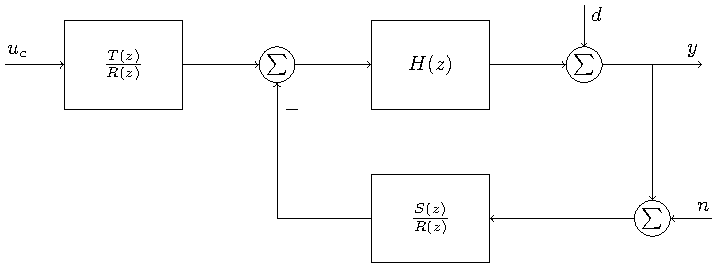
\includegraphics[width=0.7\linewidth]{../../homework/rst-block}
\caption{RST controller}
\label{fig:2dof}
\end{center}
\end{figure}

\subsection*{(b)}
\label{sec:orgheadline3}
Write a line of matlab code that computes the control signal \(u(kh)\), given the command signal \(u_c(kh)\) and the measured plant output \(y(kh)\).

\section*{Problem 2 Discretization (Å\&W problem 8.3)}
\label{sec:orgheadline7}
A continuous-time controller has been designed and is given by 
\begin{equation}
\frac{d}{dt}u  + 2u = 4\frac{d}{dt}e + 4 e
\label{eq:de}
\end{equation}

\subsection*{(a)}
\label{sec:orgheadline5}
Determine the transfer function \(F(s)\) of the controller.
\subsection*{(b)}
\label{sec:orgheadline6}
Determine a discrete-time controller \(F_d(z)\) for the sampling time \(h=\unit{0.25}{\second}\) using 
\begin{enumerate}
\item Backward difference
\item Tustin's approximation
\end{enumerate}
Find the pole of the discretetized controllers in both cases.

\section*{Problem 3 Sampling and aliasing}
\label{sec:orgheadline10}
Consider a measurement noise originating from the electrical net affecting the feedback signal in Problem 2. The noise is in the form of a sinusoid of frequency \unit{60}{\hertz}
\begin{equation}
n(t) = a \cos 120\pi t .
\end{equation}

\subsection*{(a)}
\label{sec:orgheadline8}
The signal is sampled with \(h=\unit{0.25}{s}\). What is the alias frequency in the frequency band \([0, \omega_N]\) of the noise?

\subsection*{(b)}
\label{sec:orgheadline9}
Use your favourite programming language to verify and illustrate the result in (a).

\section*{Solutions}
\label{sec:orgheadline21}
\subsection*{Problem 1}
\label{sec:orgheadline13}
\subsubsection*{(a)}
\label{sec:orgheadline11}
We have 
\[
    H(z) = \frac{B(z)}{A(z)} = \frac{1}{z + a}.
    \]
Further, we have one factor in the right hand side of the Diophantine equation given:
\[ A_{cl}(z) = A_c(z)A_o(z) = (z+\alpha) A_o(z). \]
The Diophantine equation becomes
\[ (z+a) R(z) + S(z) = (z+\alpha) A_o(z). \]
We need to decide the order of the observer polynomial in order to determine the order of the controller polynomials and then solve the Diophantine equation. 

The simplest controller is obtained with the choice \(A_o(z)=1\). This gives the equation
\[ (z+a) R(z) + S(z) = (z+\alpha). \]
Since the right hand side has order one, the left hand side must also have order one. This gives that \(R(z)\) must be of order zero. Further, \(S(z)\) cannot be of higher order than \(R(z)\), so we must have the controller polynomials
\[ R(z) = r_0, \quad S(z) = s_0. \]
We get the equation
\[ (z+a)r_0 + s_0 = (z+\alpha), \]
which leads to the equations
\begin{align}
r_0 &= 1\\
a r_0 + s_0 &= \alpha,
\end{align}
with solution
\begin{align}
r_0 &= 1\\
s_0 = \alpha-a
\end{align}

We must also determine the \(T\) polynomial. The pulse transfer function from \(u_c\) to \(y\) is given by
\[ H_c(z) = \frac{T(z)B(z)}{A_c(z)A_o(z)}. \]
From the specification, this is to be equal to 
\[ H_m(z) = \frac{1+\alpha}{z+\alpha}. \]
We have \(A_o(z) = 1\) and \(B(z) = 1\), so we get the equation
\[ \frac{T(z)}{z+\alpha} = \frac{1+\alpha}{z+\alpha}, \]
and hence
\[ T(z) = 1 + \alpha. \]

The resulting controller becomes 
\begin{align}
 R(z) U &= T(z)U_c - S(z)Y\\
 U &= (1+\alpha)U_c - (\alpha-a)Y\\
 u(kh) &= (1+\alpha)u_c(kh) - (\alpha-a)y(kh).
\end{align}
\subsubsection*{(b)}
\label{sec:orgheadline12}
The solution to (a) is a static controller, and it is straight-forward to implement this in matlab code:
\begin{verbatim}
u = (1+alpha)*u_c - (alpha-a)*y
\end{verbatim}

\subsection*{Problem 2}
\label{sec:orgheadline16}
\subsubsection*{(a)}
\label{sec:orgheadline14}
Applying the Laplace transform to both sides of the differential equation \eqref{eq:de} gives
\[ U(s) = F(s)E(s) = \frac{4(s+1)}{s+2} E(s). \]
\subsubsection*{(b)}
\label{sec:orgheadline15}
\begin{enumerate}
\item The backward approximation of the differentiation is 
\[ s = \frac{z-1}{zh} \]
which gives
\[F_d(z) = F(s)|_{s=\frac{z-1}{zh}} = 4\frac{\frac{z-1}{zh} + 1}{\frac{z-1}{zh} + 2}
                = 4\frac{z-1+zh}{z-1 + 2zh} = 4\frac{(1+h)z - 1}{(1+2h)z - 1}. \]
with \(h=0.25\) we get
\[ F_d(z) = 4\frac{1.25z - 1}{1.5z - 1}, \]
which has a pole in \(z=2/3\).
\item Tustin's approximation of the differentiation is 
\[ s = \frac{2}{h}\frac{z-1}{z+1} \]
which gives
\[F_d(z) = F(s)|_{s=\frac{2}{h}\frac{z-1}{z+1}} = 4\frac{\frac{2}{h}\frac{z-1}{z+1} + 1}{\frac{2}{h}\frac{z-1}{z+1} + 2}
                = 4\frac{2(z-1) + h(z+1)}{2(z-1) + 2h(z+1)} = 4\frac{(2+h)z - (2-h)}{(2+2h)z -(2-2h)}. \]
with \(h=0.25\) we get
\[ F_d(z) = 4\frac{2.25z - 1.75}{2.5z - 1.5}, \]
which has a pole in \(z=3/5\).
\end{enumerate}

\subsection*{Problem 3}
\label{sec:orgheadline20}

\subsubsection*{(a)}
\label{sec:orgheadline18}
We have sampling time \(h=\unit{0.25}{\second}\) and so the sampling frequency in \unit{}{\rad\per\second} is
\[\omega_s = \frac{2\pi}{h} = \frac{2\pi}{0.25} = 8 \pi, \]
and the Nyquist frequncy is 
\[ \omega_N = \omega_s/2 = 4 \pi. \]

The sampled noise signal will have Fourier transform
\[ F_s(\omega) = \sum_{k=-\infty}^\infty F(\omega + k\omega_s), \]
where the Fourier transform of the noise is 
\[ F(\omega) =  a\pi\left( \delta(\omega + \omega_1) - \delta(\omega - \omega_1) \right) \]
Since the Fourier transform of the sinusoid is zero except at the two frequencies \(\omega = \omega_1\) and \(\omega=-\omega_1\), the Fourier transform of the sampled signal will be zero expect at all frequencies \(\omega\) such that
\[ \omega + k\omega_s = \omega_1 \quad \Rightarrow \quad \omega = \omega_1 + k\omega_s\]
and
\[ \omega + k\omega_s = -\omega_1 \quad \Rightarrow \quad \omega = -\omega_1 + k\omega_s.\]

Hence, the alias frequencies of the noise frequency \(\omega_1 = 120\pi\) will be the set
\[ \{\omega_1 \pm k\omega_s\,|\, k=0,1,\ldots \} \; \cup \; \{-\omega_1 \pm k\omega_s\,|\, k=0,1,\ldots \} \]

To find the alias frequency in the band \([0, \omega_N]\), we solve for integer solutions \(k\) to the inequalities
\[ 0 \le \omega_1 + k\omega_s \le \omega_N \]
and
\[ 0 \le -\omega_1 + k\omega_s \le \omega_N. \]
This gives for the first inequality
\[ 0 \le 120\pi + k8\pi \quad \Rightarrow \quad k \ge -\frac{120}{8} = -15, \]
\[ 120\pi + k8\pi \le 4\pi \quad \Rightarrow \quad k \le -\frac{116}{8} = -14.5. \]
\(k\) must be integer-valued, so we have
\[ k = -15, \]
with alias frequency
\[ \omega_a = \omega_1 - 15\omega_s = 120\pi - 15\cdot 8 \pi = 0. \]

For the second inequality we get
\[ 0 \le -120\pi + k8\pi \quad \Rightarrow \quad k \ge \frac{120}{8} = 15, \]
\[ -120\pi + k8\pi \le 4\pi \quad \Rightarrow \quad k \le \frac{124}{8} = 15.5. \]
Again, \(k\) must be integer valued, and we get 
\[ k = 15, \]
with alias frequency
\[ \omega_a = -\omega_1 + 15\omega_s = -120\pi + 15\cdot 8 \pi = 0. \]

The sampling of the \unit{60}{\hertz} noise at \(h=\unit{0.25}{\second}\) gives a constant alias signal (bias) to the sampled feedback signal. The size of the bias depends on the magnitude \(a\) of the sinusoid, as well as the phase of the sinusoid at the sampling instants.


\begin{itemize}
\item Alternative solution.
\label{sec:orgheadline17}
It is quite a bit faster to apply equation (7.10) in Å\&W directly. This gives for the alias frequency
\begin{equation*}
 \begin{split}
  \omega_a &= | (\omega_1 + \omega_N) \mod \omega_s - \omega_N| \\
	   &= | (120\pi + 4\pi) \mod 8\pi - 4\pi | = |4\pi - 4\pi| = 0.
 \end{split}
\end{equation*}
\end{itemize}
\subsubsection*{(b)}
\label{sec:orgheadline19}
Using python. See \url{https://github.com/alfkjartan/control-computarizado/blob/master/partial2-prep-aliasing-spring16.ipynb}
\end{document}
